\documentclass[tikz,border=5pt]{standalone}
\usepackage{tikz}
\usepackage{graphicx}
\pagestyle{empty}
\begin{document}
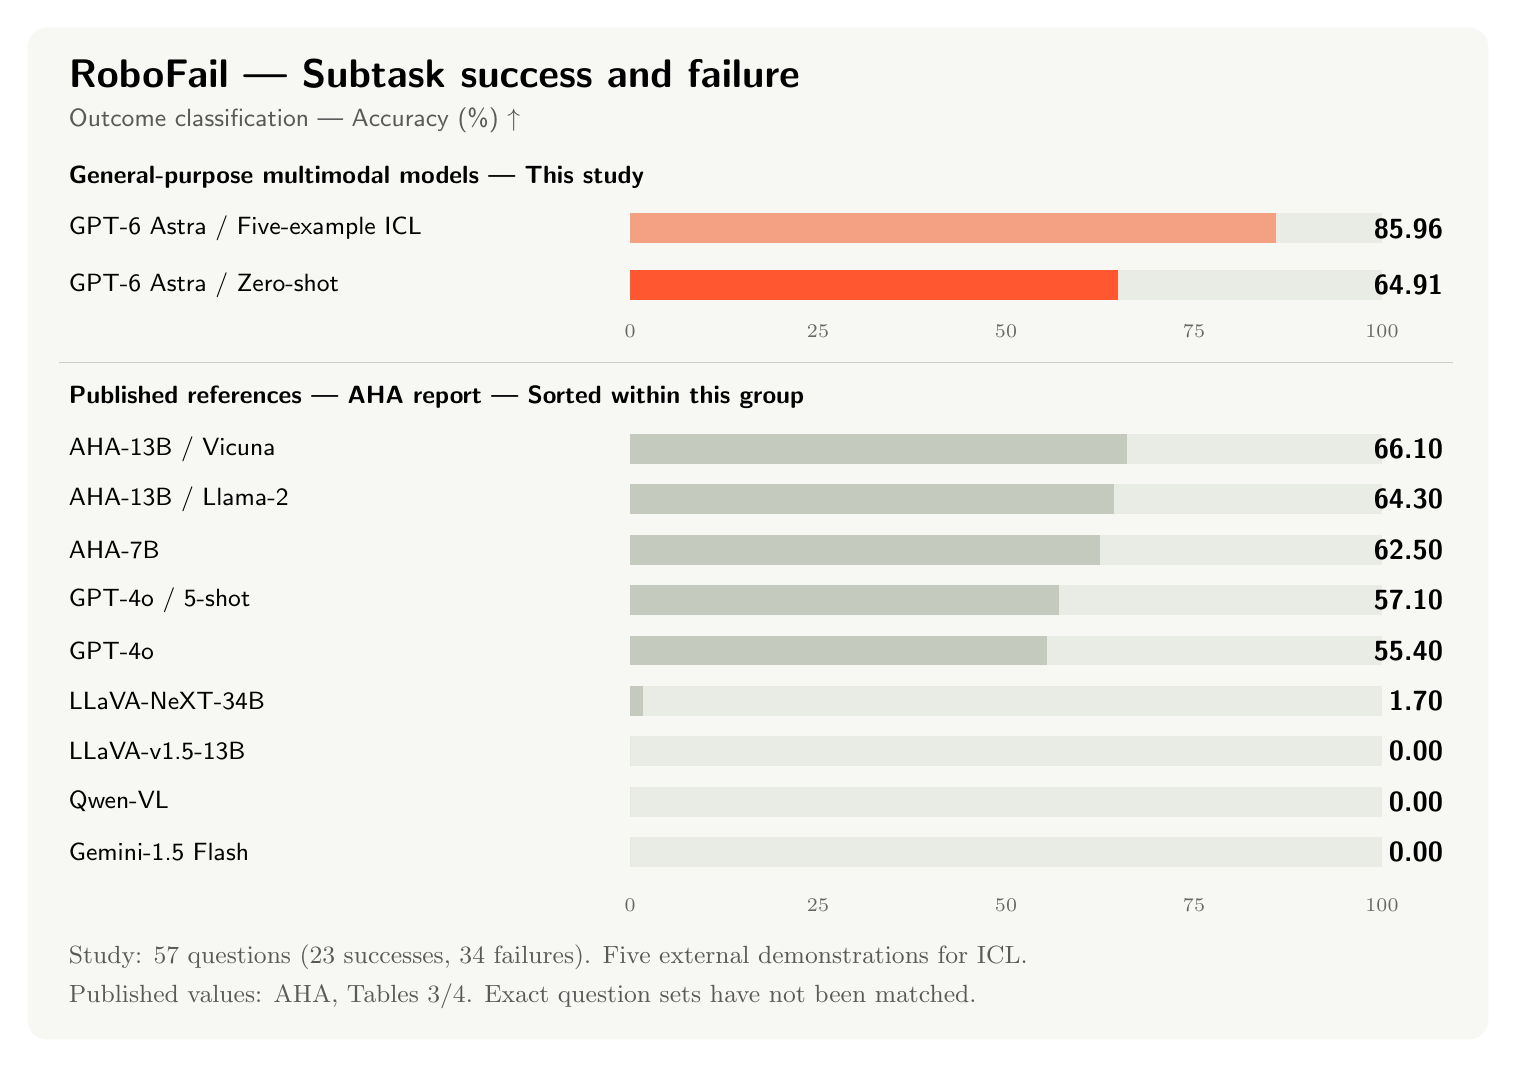
\begin{tikzpicture}[x=1cm,y=1cm,font=\sffamily]
\definecolor{cardbg}{HTML}{F7F8F3}
\definecolor{trackbg}{HTML}{E9ECE4}
\definecolor{mutedbar}{HTML}{C5CABF}
\definecolor{astrabar}{HTML}{FF572F}
\definecolor{iclbar}{HTML}{F4A082}
\definecolor{studybar}{HTML}{79958A}
\fill[cardbg,rounded corners=7pt] (-.4,2) rectangle (18.15,-10.85);
\node[anchor=west,font=\sffamily\bfseries\Large] at (0,1.42) {RoboFail | Subtask success and failure};
\node[anchor=west,font=\sffamily\small,text=black!65] at (0,.82) {Outcome classification | Accuracy (\%) $\uparrow$};
\node[anchor=west,font=\sffamily\bfseries\small] at (0,.1) {General-purpose multimodal models | This study};
\node[anchor=west,font=\sffamily\small] at (0,-0.55) {GPT-6 Astra / Five-example ICL};
\fill[trackbg] (7.25,-0.74) rectangle (16.8,-0.36);
\fill[iclbar] (7.25,-0.74) rectangle (15.459180,-0.36);
\node[anchor=east,font=\sffamily\bfseries] at (17.7,-0.55) {85.96};
\node[anchor=west,font=\sffamily\small] at (0,-1.27) {GPT-6 Astra / Zero-shot};
\fill[trackbg] (7.25,-1.46) rectangle (16.8,-1.08);
\fill[astrabar] (7.25,-1.46) rectangle (13.448905,-1.08);
\node[anchor=east,font=\sffamily\bfseries] at (17.7,-1.27) {64.91};
\node[text=black!60,font=\scriptsize] at (7.25,-1.85) {0};
\node[text=black!60,font=\scriptsize] at (9.6375,-1.85) {25};
\node[text=black!60,font=\scriptsize] at (12.025,-1.85) {50};
\node[text=black!60,font=\scriptsize] at (14.4125,-1.85) {75};
\node[text=black!60,font=\scriptsize] at (16.8,-1.85) {100};
\draw[black!20] (0,-2.25) -- (17.7,-2.25);
\node[anchor=west,font=\sffamily\bfseries\small] at (0,-2.7) {Published references | AHA report | Sorted within this group};
\node[anchor=west,font=\sffamily\small] at (0,-3.35) {AHA-13B / Vicuna};
\fill[trackbg] (7.25,-3.54) rectangle (16.8,-3.16);
\fill[mutedbar] (7.25,-3.54) rectangle (13.562550,-3.16);
\node[anchor=east,font=\sffamily\bfseries] at (17.7,-3.35) {66.10};
\node[anchor=west,font=\sffamily\small] at (0,-3.99) {AHA-13B / Llama-2};
\fill[trackbg] (7.25,-4.18) rectangle (16.8,-3.80);
\fill[mutedbar] (7.25,-4.18) rectangle (13.390650,-3.80);
\node[anchor=east,font=\sffamily\bfseries] at (17.7,-3.99) {64.30};
\node[anchor=west,font=\sffamily\small] at (0,-4.63) {AHA-7B};
\fill[trackbg] (7.25,-4.82) rectangle (16.8,-4.44);
\fill[mutedbar] (7.25,-4.82) rectangle (13.218750,-4.44);
\node[anchor=east,font=\sffamily\bfseries] at (17.7,-4.63) {62.50};
\node[anchor=west,font=\sffamily\small] at (0,-5.27) {GPT-4o / 5-shot};
\fill[trackbg] (7.25,-5.46) rectangle (16.8,-5.08);
\fill[mutedbar] (7.25,-5.46) rectangle (12.703050,-5.08);
\node[anchor=east,font=\sffamily\bfseries] at (17.7,-5.27) {57.10};
\node[anchor=west,font=\sffamily\small] at (0,-5.91) {GPT-4o};
\fill[trackbg] (7.25,-6.10) rectangle (16.8,-5.72);
\fill[mutedbar] (7.25,-6.10) rectangle (12.540700,-5.72);
\node[anchor=east,font=\sffamily\bfseries] at (17.7,-5.91) {55.40};
\node[anchor=west,font=\sffamily\small] at (0,-6.55) {LLaVA-NeXT-34B};
\fill[trackbg] (7.25,-6.74) rectangle (16.8,-6.36);
\fill[mutedbar] (7.25,-6.74) rectangle (7.412350,-6.36);
\node[anchor=east,font=\sffamily\bfseries] at (17.7,-6.55) {1.70};
\node[anchor=west,font=\sffamily\small] at (0,-7.19) {LLaVA-v1.5-13B};
\fill[trackbg] (7.25,-7.38) rectangle (16.8,-7.00);
\fill[mutedbar] (7.25,-7.38) rectangle (7.250000,-7.00);
\node[anchor=east,font=\sffamily\bfseries] at (17.7,-7.19) {0.00};
\node[anchor=west,font=\sffamily\small] at (0,-7.83) {Qwen-VL};
\fill[trackbg] (7.25,-8.02) rectangle (16.8,-7.64);
\fill[mutedbar] (7.25,-8.02) rectangle (7.250000,-7.64);
\node[anchor=east,font=\sffamily\bfseries] at (17.7,-7.83) {0.00};
\node[anchor=west,font=\sffamily\small] at (0,-8.47) {Gemini-1.5 Flash};
\fill[trackbg] (7.25,-8.66) rectangle (16.8,-8.28);
\fill[mutedbar] (7.25,-8.66) rectangle (7.250000,-8.28);
\node[anchor=east,font=\sffamily\bfseries] at (17.7,-8.47) {0.00};
\node[text=black!60,font=\scriptsize] at (7.25,-9.15) {0};
\node[text=black!60,font=\scriptsize] at (9.6375,-9.15) {25};
\node[text=black!60,font=\scriptsize] at (12.025,-9.15) {50};
\node[text=black!60,font=\scriptsize] at (14.4125,-9.15) {75};
\node[text=black!60,font=\scriptsize] at (16.8,-9.15) {100};
\node[anchor=west,text=black!65,font=\small] at (0,-9.8) {Study: 57 questions (23 successes, 34 failures). Five external demonstrations for ICL.};
\node[anchor=west,text=black!65,font=\small] at (0,-10.3) {Published values: AHA, Tables 3/4. Exact question sets have not been matched.};
\end{tikzpicture}
\end{document}
